\documentclass[11pt]{article}
\usepackage[margin=2.5cm]{geometry}
\usepackage{graphicx,booktabs,hyperref,amsmath}
\usepackage[T1]{fontenc}
\hypersetup{colorlinks=true,linkcolor=black,urlcolor=blue,citecolor=black}
\newcommand{\as}{$''$}
\title{(1036) Ganymed on Harvard plates of 1898, 26 years before its discovery, and a candidate image of (624) Hektor from 1901}
\author{Qianghao Wu}
\date{November 27, 2026}
\begin{document}
\sloppy
\maketitle

\begin{abstract}
The earliest observation of the near-Earth asteroid (1036) Ganymed in the JPL Small-Body Database and in the Minor Planet Center observation list is its discovery on 1924 Oct 23. We searched the public scans of six Harvard plates of 1898--1899 for it with a test that we registered in advance: plates, predicted positions, statistic and decision rule were committed before any image was downloaded. Three of the six plates pass the per-plate threshold (i21050 of 1898 Aug 14, i21576 of 1898 Nov 1 and i21780 of 1898 Nov 26). The probability of three or more passes under the per-plate null rates, which come from 300 random regions on each plate, is $5.1\times10^{-4}$, below the registered threshold of $10^{-3}$. A source is at the predicted position on five plates. Their measured positions are 0.4\as{} to 2.4\as{} from the JPL Horizons ephemeris, and they are up to $97^\circ$ apart on the sky. On i21050 the result depends on the centroid method (2.4\as{} to 13.5\as{}). The images are 26 years older than the discovery. A second, weaker result concerns the Jupiter Trojan (624) Hektor, whose earliest catalogued observation is 1907 Feb 11; the earliest catalogued observation of any Jupiter Trojan is 1904 Sep 13. Two registered searches of Harvard plates did not detect Hektor. A third registered search, of 15 Heidelberg plates, passed its rule: three plates of 1901 Aug 23 give $p=0.0015$, 0.0050 and 0.0065 (Fisher $p=1.5\times10^{-5}$). An independent measurement gives larger values ($p=0.009$, 0.023, 0.040; Fisher $6.6\times10^{-4}$), and all three plates are from one night. We therefore report the Hektor signal as a candidate detection only. Neither result has been checked on the glass plates.
This work has not yet been reviewed by experts. The computations and the text were produced by AI models (from Anthropic and OpenAI), working under the author's direction.
\end{abstract}

\section{Introduction}
(1036) Ganymed is the largest known near-Earth asteroid. W.~Baade discovered it at Bergedorf on 1924 Oct 23 (designation A924~UB)~\cite{sbdb}. In the JPL Small-Body Database (SBDB) its first observation (\texttt{first\_obs}) is the discovery date, 1924-10-23~\cite{sbdb}. In the Minor Planet Center (MPC) observation list, the earliest observation of Ganymed is 1924 Oct 23.809~\cite{mpcobs}. The MP3C database gives the years observed as 1924--2023~\cite{mp3c}.

A \emph{precovery} is an image of an object on a plate or a frame that was taken before its discovery. The Harvard College Observatory plate collection is now public in digital form through DASCH (Digital Access to a Sky Century @ Harvard)~\cite{grindlay2012,dasch}. Recent precovery work on DASCH plates includes a search for the distant object 2026~ED$_{138}$ by Murtagh et al.~\cite{murtagh2026}, candidate images of Pluto on plates of 1908--1909 by Graham~\cite{graham2026}, and a time error in the DASCH metadata of J.\,H.~Metcalf's plates with Pluto on four plates of 1908--1909~\cite{wu2026metcalf}. None of these concerns Ganymed or Hektor.

We found no image of Ganymed earlier than 1924 in the SBDB, the MPC list, MP3C, a web search, the two public collections of AI-produced research results, the archives where such results are posted, or Zenodo (searches of 2026 Nov 27). These searches do not cover all plate archives. Ganymed's orbit is already well determined, so the scientific gain of the 1898 positions is small. The value of the result is the record and the method.

(624) Hektor is a Jupiter Trojan. A.~Kopff discovered it at Heidelberg on 1907 Feb 10 (designation A907~CF)~\cite{sbdb}. Its SBDB \texttt{first\_obs} is 1907-02-11. An SBDB query for all Jupiter Trojans with \texttt{first\_obs} before 1907 Mar 1 returns four objects. The earliest is (12126) Chersidamas, 1904-09-13; then (588) Achilles, (617) Patroclus and Hektor~\cite{sbdb}. The MPC list has no Hektor observation before 1907 Feb 11.021 and no Chersidamas observation before 1904 Sep 13.174~\cite{mpcobs}. An image of Hektor before 1904 Sep 13 would be the earliest known image of a Jupiter Trojan. Heidelberg plates are public through the HDAP archive (Heidelberg Digitized Astronomical Plates)~\cite{hdap}. Web searches of 2026 Nov 27 found no image of Hektor before 1907.

\section{Data}
\begin{itemize}
\item \textbf{DASCH DR7}~\cite{dasch}: plate metadata, cutouts of the plate scans ($835\times835$ pixels, 1.44\as{} per pixel) and the plate WCS, through the public API (\url{https://api.starglass.cfa.harvard.edu/public}). The API also serves ATLAS-REFCAT2 stars~\cite{tonry2018} for a sky region. Accessed 2026 Nov 27.
\item \textbf{HDAP}~\cite{hdap}: the plate table \texttt{lsw.plates} through the TAP service of the GAVO Data Center and cutouts of radius $0.2^\circ$ through its SODA service. Licence CC0~1.0. Accessed 2026 Nov 27.
\item \textbf{JPL Horizons}~\cite{horizons}: topocentric astrometric positions (ICRF) and the predicted V magnitude for MPC sites 800 (Arequipa), 802 (Cambridge, Massachusetts) and 024 (Heidelberg). We use the SBDB orbit that Horizons served on 2026 Nov 27.
\end{itemize}

\section{Method}
\subsection{Registration}
The protocol (\texttt{PROTOCOL.md} in the result folder) is in git. Its commit time is the evidence that the rules came before the data. Table~\ref{tab:prereg} gives each registration commit and the first download after it. The full commit list is in \texttt{data/GIT\_LOG.txt}.

\begin{table}[h]
\centering\small
\begin{tabular}{llll}\toprule
Round & Commit & Commit time (CET) & First cutout request (CET) \\\midrule
1 (Ganymed, Hektor) & \texttt{c64fc2c} & 2026-11-27 14:07:44 & 14:07:49 \\
2 (Hektor) & \texttt{907bdc5} & 2026-11-27 14:28:05 & 14:28:05 \\
3 (Hektor, HDAP) & \texttt{a01e3ff} & 2026-11-27 15:00:43 & 15:01:22 \\\bottomrule
\end{tabular}
\caption{Registration commits. The request times of rounds 1 and 2 are in the DASCH request log (\texttt{data/cutouts/log.jsonl}). Round 3 was done in a separate copy of the repository. Its original commit is \texttt{69a64b8}; in the published repository it is the cherry-pick \texttt{a01e3ff}, with author date 15:00:43 and committer date 16:01:23. The author date is the registration time. The HDAP request log has no time stamps; the time of the first round-3 cutout (15:01:22) is the file time in the separate copy, read by the verification stage.}
\label{tab:prereg}
\end{table}

\subsection{Round 1: plates and predictions}
The plate list is in \texttt{src/plates.py}. The rule: DASCH DR7 plates taken before the object's first observation, with the object inside the plate, and with limiting magnitude minus $(V+0.8)$ above 0.3, where 0.8 is an assumed $B-V$. It gives six Ganymed plates of the i and ac series (Cambridge, 1898 Aug 14 to 1899 Jan 20) and five Hektor plates of the b series (Arequipa, 1899--1901). For each plate, \texttt{src/predict.py} takes the Horizons position every 5~min from the DASCH midpoint $-2$\,h to $+2$\,h. The Sun is below $-24^\circ$ at all midpoints.

\subsection{Round 1: statistic and decision}
\texttt{src/measure.py} makes a noise-normalised image $z$: the scan smoothed with a Gaussian of 1.5 pixels, minus the scan smoothed with a Gaussian of 15 pixels, divided by the robust standard deviation. It refits the plate WCS to the ATLAS stars where enough stars match. The search region is the predicted track within $\pm1$\,h of the midpoint, with a buffer of 15\as{} (Ganymed) or 10\as{} (Hektor). Catalogued stars are masked. The statistic $S$ is the maximum of $z$ in the region. A plate passes if $S\ge10$ (Ganymed) or $S\ge6$ (Hektor). The null rate $p_0$ of each plate is the fraction of 300 copies of the region, at random offsets of 90\as{} to 420\as{} on the same cutout, that pass. An object is \emph{detected} if at least two plates pass and the Poisson-binomial probability $P$ of at least that many passes under the $p_0$ values is below $10^{-3}$.

\subsection{Rounds 2 and 3 (Hektor)}
Round~2 used the eight other DASCH plates before 1907 Feb 11 that satisfy a looser magnitude rule. The statistic is the maximum of $z$ within 5\as{} of the predicted midpoint position, with $p$ from 2000 random unmasked points on the same cutout. The decision: Fisher combination $p_{\rm comb}<10^{-3}$ and at least two plates with $p<0.01$.

Round~3 used the HDAP plates of 1895--1907. \texttt{src/hdap\_cover.py} found 18 of 3857 plates with a coverage polygon that contains Hektor; three plates with Hektor less than $0.1^\circ$ from the edge were removed, which leaves 15. The HDAP plate times are uncertain: on plate G2392 the header UT and the header sidereal time differ by 45~min. The statistic of \texttt{src/hdap.py} is therefore the mean $z$ along the predicted trail, maximised over time shifts from $-60$ to $+60$\,min. The null is 2000 random translations (90\as{} to 600\as{}) of the same trail family on the same plate, with the same maximisation. The decision rule is the round-2 rule, applied to set~A (plates before 1904 Sep 13) and set~B (all plates).

\subsection{Changes after registration}\label{sec:changes}
All changes are dated addenda in \texttt{PROTOCOL.md}. One change touched a registered input. A Horizons row with a rise, transit or set mark has one CSV field less. The registered parser dropped such rows. For plate i21780 the dropped row was the midpoint row, so the registered prediction was the position 5~min later, 5.5\as{} away. The corrected parser (\texttt{src/hz.py}) reads these rows, and \texttt{src/predict.py} stops if no row is at the DASCH midpoint. The corrected i21780 cutout and the registered one are both kept. The registered result (\texttt{data/prereg/results.json}) and the corrected result (\texttt{data/results.json}) give the same decision; i21780 has $S=16.0$ in both. Round~2 is identical. In round~3, Addendum 5 added a row filter as a work-around for the same defect, and Addendum 7 removed it again. No midpoint changed, and all 15 $p$ values are identical.

\subsection{Astrometry and shapes (after the decision)}
\texttt{src/astrometry.py} measures the position of the source after the decision. This is a measurement, not a test. The main method (``region'') takes the intensity-weighted centroid of the whole region above half maximum, for the source and for the reference stars brighter than the plate limit minus 1~mag. With fewer than six stars the model is a shift of the DASCH WCS; with six or more it is affine. The second method (``box'') takes an $11\times11$ pixel box centroid and stars to the limit plus 0.3~mag. The O$-$C is the difference from the Horizons position at the DASCH midpoint. The along-track part divided by the rate of motion gives an equivalent time offset. \texttt{src/shapes.py} measures the position angle (PA) and the length of the half-maximum region of the source and of stars on the same cutout.

\section{Result: Ganymed}
Table~\ref{tab:ganymed} gives the registered test. Three of six plates pass. $P=5.07\times10^{-4}<10^{-3}$: Ganymed is \emph{detected} by the registered rule. The earliest passing plate is i21050, 1898 Aug 14, 07:12~UT (DASCH midpoint). On two plates no control region passed ($p_0=0$). With a floor of $1/300$ for these plates, $P=6.25\times10^{-4}$.

\begin{table}[h]
\centering\small
\begin{tabular}{llrrrrl}\toprule
Plate & DASCH midpoint (UT) & Exp.\ (min) & $V$ & Limit & $S$ & $p_0$ \\\midrule
i21050 & 1898-08-14 07:12 & 14 & 10.0 & 13.9 & 23.3 & 0.043 (pass) \\
ac00044 & 1898-09-21 05:31 & 94 & 9.0 & 12.4 & 3.6 & 0 \\
i21576 & 1898-11-01 05:01 & 12 & 8.4 & 13.6 & 33.1 & 0.163 (pass) \\
i21780 & 1898-11-26 02:12 & 13 & 10.0 & 13.4 & 16.0 & 0.030 (pass) \\
ac00115 & 1898-12-10 01:45 & 63 & 10.8 & 13.6 & 9.3 & 0.023 \\
i22152 & 1899-01-20 01:07 & 10 & 12.4 & 13.6 & 5.4 & 0 \\\bottomrule
\end{tabular}
\caption{Round 1, Ganymed. $V$: Horizons magnitude. Limit: DASCH limiting magnitude. Pass: $S\ge10$.}
\label{tab:ganymed}
\end{table}

\begin{figure}[t]
\centering
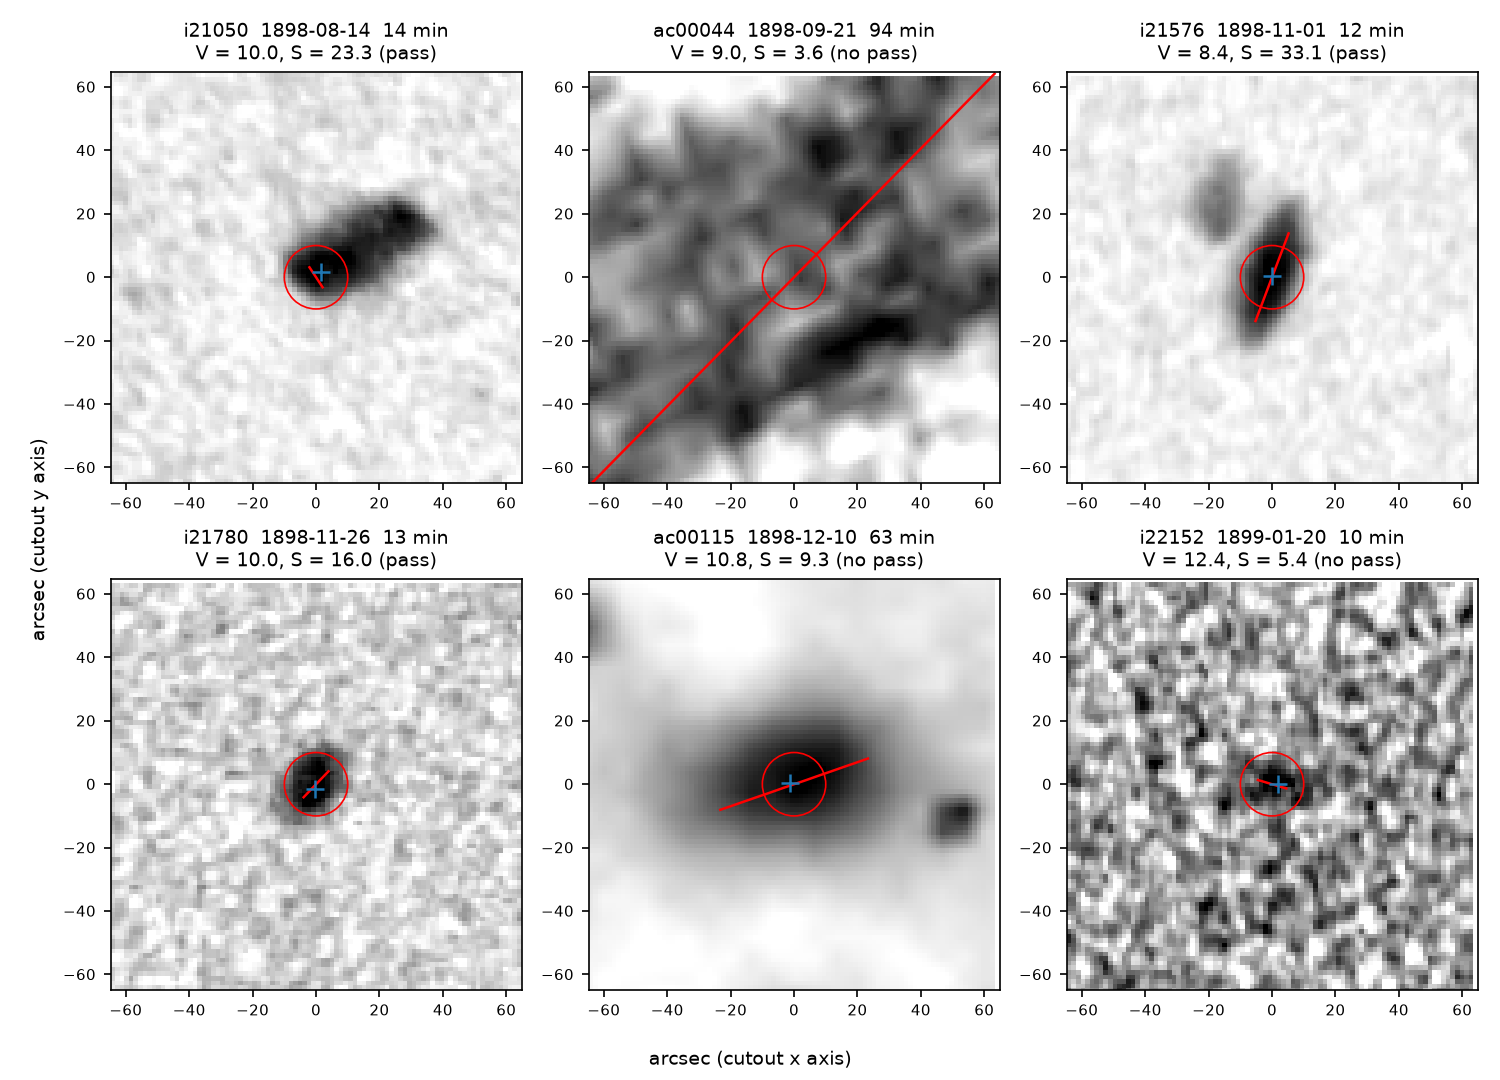
\includegraphics[width=0.92\textwidth]{fig_ganymed.png}
\caption{The six Ganymed plates of round 1, $130''\times130''$, centred on the predicted midpoint position. Red line: predicted motion during the exposure. Red circle: radius 10\as. Blue cross: measured position (region method). The star images on i21050 are also elongated (median length 43\as{} along PA $28^\circ$), so the source there has the shape of a star. On ac00044 the registered test fails; we make no claim for that plate.}
\label{fig:ganymed}
\end{figure}

\paragraph{The plates that do not pass.} On ac00115 ($S=9.3$) a source is at the predicted position (Figure~\ref{fig:ganymed}). On i22152 ($S=5.4$) the source alone is weak; its support is its position (O$-$C 1.9\as). On ac00044 ($S=3.6$) the expected image is a 189\as{} trail on a plate with star images about 20\as{} long. The verification stage found a broad feature on the predicted trail; its nature is not known. We make no claim for ac00044.

\paragraph{Astrometry.} Table~\ref{tab:ast} gives the positions. The region method gives O$-$C from 0.36\as{} to 2.36\as; the equivalent time offsets are $-2.0$ to $+1.3$~min. The box method gives 1.26\as, 0.92\as, 3.12\as, 4.24\as{} and 1.06\as, with time offsets of $-4.8$ to $+2.3$~min. On ac00115 the box (16\as) is shorter than the 52\as{} trail, so its along-track value depends on the start point. The region method has two free choices: the star match tolerance (4, 8 or 12 pixels) and the faint limit of the reference stars. Over the six combinations the O$-$C is 2.36\as--13.47\as{} on i21050, 0.36\as--1.59\as{} on i21576, 1.66\as--2.40\as{} on i21780, 1.28\as--1.50\as{} on ac00115 and 1.65\as--1.91\as{} on i22152. On i21050 the bright stars have asymmetric images, and the centroid definition moves the result by up to 11\as. The i21050 position is therefore uncertain by several arcseconds. The Horizons $3\sigma$ uncertainty of Ganymed in 1898 is below 0.7\as{} in RA and below 0.2\as{} in Dec (verification stage). The O$-$C values are therefore measurement errors of the old plates, not ephemeris errors.

\begin{table}[h]
\centering\small
\begin{tabular}{lllrrrrr}\toprule
Plate & Model & Stars & RA (deg) & Dec (deg) & O$-$C RA$\cos\delta$ & O$-$C Dec & O$-$C \\\midrule
i21050 & affine & 12 & 310.42014 & $+63.18816$ & $-1.57$ & $+1.76$ & 2.36 \\
i21576 & shift & 2 & 18.10586 & $+13.42383$ & $+0.14$ & $+0.33$ & 0.36 \\
i21780 & shift & 1 & 27.44422 & $-3.37493$ & $+0.39$ & $-1.61$ & 1.66 \\
ac00115 & shift & 2 & 32.02686 & $-6.26578$ & $+1.25$ & $+0.31$ & 1.29 \\
i22152 & shift & 2 & 46.12271 & $-4.95514$ & $-1.91$ & $-0.06$ & 1.91 \\\bottomrule
\end{tabular}
\caption{Positions of the source (region method, ICRF, at the DASCH midpoint) and O$-$C against Horizons in arcseconds. Stars: number of ATLAS reference stars in the fit.}
\label{tab:ast}
\end{table}

\paragraph{A moving source.} The five positions are up to $97.0^\circ$ apart on the sky. A star or a plate flaw cannot follow the track. No catalogued star brighter than 13.8~mag is within 30\as{} of any prediction. The verification stage looked at four other i-series plates of other dates that cover the i21050, i21576 and i21780 positions. The maximum $z$ within 17\as{} of the position is 1.5 to 2.3 on these plates; no source is there.

\paragraph{Shapes.} On i21050, i21780 and i22152 the predicted motion during the exposure (11\as, 15\as{} and 9\as) is shorter than a star image, and the source has the shape of the stars on the same plate. On i21576 the source is 39\as{} long at PA $72^\circ$; the predicted trail is 35\as{} at PA $69^\circ$. On ac00115 the source is 54\as{} long at PA $10^\circ$; the predicted trail is 52\as{} at PA $19^\circ$. These two sources are longer than the stars, but only one and three comparison stars exist on these plates, and their images are also elongated in a similar direction. The shapes are consistent with a moving object. They do not prove it.

\section{Result: Hektor (candidate)}
Table~\ref{tab:rounds} summarises the three registered rounds.

\begin{table}[h]
\centering\small
\begin{tabular}{lp{3.2cm}p{2.4cm}p{7.2cm}}\toprule
Round & Plates & Statistic & Result \\\midrule
1 & 5 Harvard b plates & max $z$ on the track & 2 of 5 pass (b28276 1901 Aug 23, b28503 1901 Sep 10); $P=0.029$: not detected \\
2 & 8 other Harvard plates & $z$ within 5\as{} & $p_{\rm comb}=0.0028$, no plate $p<0.01$: not detected \\
3 & 15 Heidelberg plates & trail-mean $z$ & set A: $p_{\rm comb}=1.5\times10^{-5}$, 3 plates $p<0.01$: detected \\\bottomrule
\end{tabular}
\caption{The three Hektor rounds. In round 2, a06535 does not cover the position and b23969 is inside a star mask; six plates are measurable.}
\label{tab:rounds}
\end{table}

\paragraph{Round 3.} Set A has five measurable plates (Table~\ref{tab:hdap}). B262a returned no cutout (HTTP 204). G963 and G1139 have fewer than three matched stars, so their plate WCS was used. The three plates of 1901 Aug 23 have $p<0.01$, and Fisher $p_{\rm comb}=1.49\times10^{-5}$: set A is \emph{detected} by the registered rule. With a factor 3 for the three Hektor rounds, $4.5\times10^{-5}$. This factor corrects for the number of rounds. It does not correct for the choice of the round-3 statistic, which we made after rounds 1 and 2 had failed. Set B (14 measurable plates) gives $p_{\rm comb}=3.2\times10^{-6}$. None of the nine plates of 1904 Nov--Dec has $p<0.01$ (lowest: G3623, 0.011).

\begin{table}[h]
\centering\small
\begin{tabular}{llrrrrrr}\toprule
Plate & Start (UT, header) & Exp.\ (h) & Trail (\as) & Fit stars & $S$ & $p$ & $p$ (verifier) \\\midrule
G963 & 1895-02-14 20:24 & 3.77 & 83 & WCS, 2 & 0.24 & 0.40 & -- \\
G1139 & 1896-03-15 20:46 & 2.50 & 54 & WCS, 0 & 0.76 & 0.091 & -- \\
G2281 & 1901-08-23 22:11 & 1.33 & 27 & 15 & 2.99 & 0.0015 & 0.0087 \\
G2282 & 1901-08-23 22:11 & 2.87 & 57 & 14 & 1.35 & 0.0050 & 0.0232 \\
G2283 & 1901-08-23 23:43 & 1.33 & 27 & 15 & 1.82 & 0.0065 & 0.0402 \\\bottomrule
\end{tabular}
\caption{Round 3, set A (Heidelberg, Wolf double astrograph). $S$: trail-mean $z$, maximised over time shifts. Last column: the independent measurement of the verification stage, with the same time-shift search.}
\label{tab:hdap}
\end{table}

\paragraph{How much the result depends on the analysis.} The verification stage measured the three 1901 plates with its own code: its own $z$ image, its own star fit (13--18 stars, rms 2.2\as--2.7\as), no star mask and 4000 random translations. It finds the signal on all three plates, with trail-mean $z$ of 2.35, 1.35 and 1.56 at the header time. Its $p$ values are larger (Table~\ref{tab:hdap}). With these values only one plate has $p<0.01$, so the second condition of the registered rule is not met, and the Fisher $p$ is $6.6\times10^{-4}$ (three plates) or $8.3\times10^{-4}$ (with G963 and G1139). Without the time-shift search, the verifier's $p$ values are 0.0060, 0.0125 and 0.0167 (Fisher $1.3\times10^{-4}$; $2.0\times10^{-4}$ with five plates). The Hektor signal is therefore a candidate detection that depends on the analysis choices.

\paragraph{Time shifts.} The trail-mean $z$ as a function of time shift has its maximum at $-20$~min (G2281), $+10$~min (G2282) and $+5$~min (G2283) in the verifier's measurement. These profiles are 60 to 100~min wide. The data give no measurable clock offset for these plates. The time-shift search costs sensitivity: the verifier's $p$ values are 1.5 to 2.4 times larger with it than without it.

\paragraph{Same night, two lenses.} G2281 and G2282 started 5~s apart on the same instrument, the Wolf double astrograph. They have different pixel scales (2.555\as{} and 2.503\as{} per pixel) and different star fits, so they are two glass plates from the two lenses. Their grain noise is independent. Light that reaches both lenses, for example sky background or ghost images of bright stars, can still be common to both. G2283 is a later exposure of the same night. All three plates are from one night, so they do not show the motion of Hektor from night to night.

\begin{figure}[t]
\centering
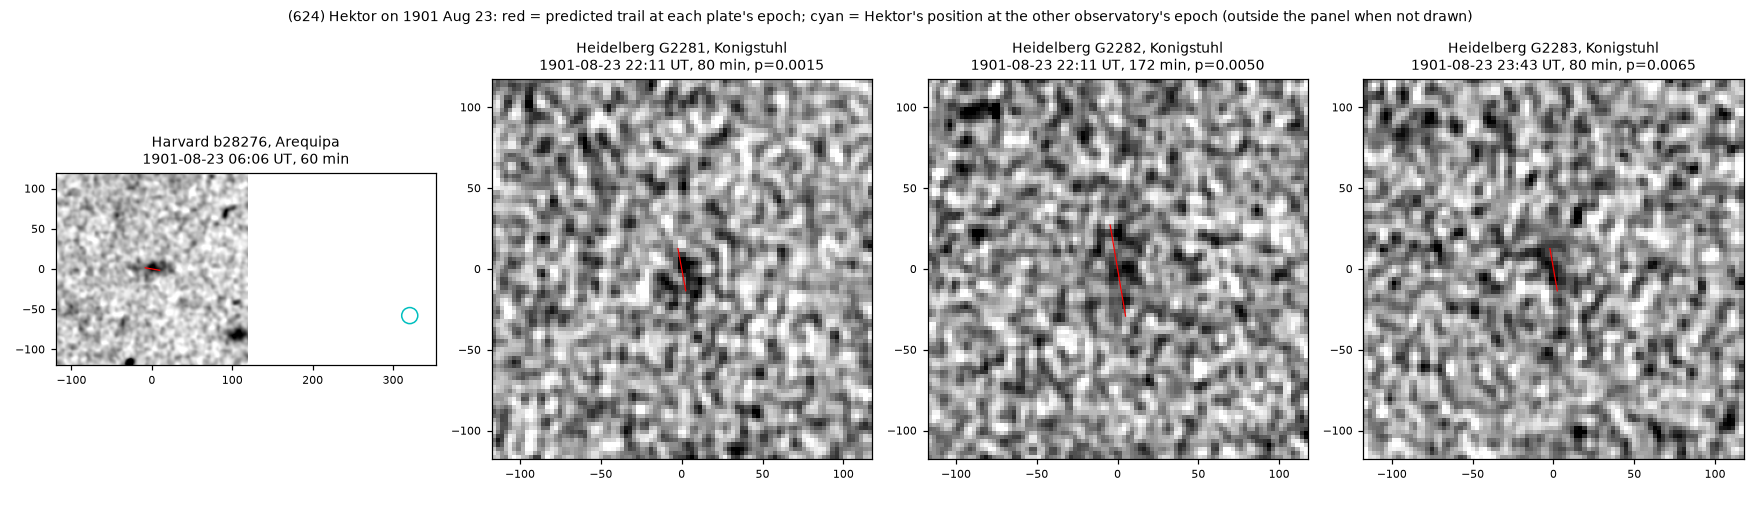
\includegraphics[width=\textwidth]{fig_hektor.png}
\caption{Hektor on 1901 Aug 23. Left: Harvard b28276 (Arequipa, 06:06 UT, round 1). Right: the three Heidelberg plates of round 3 (evening of the same date). Red: predicted trail at each plate's epoch. Cyan: Hektor's position at the other observatory's epoch, 326\as{} away. Axes in arcseconds.}
\label{fig:hektor}
\end{figure}

\paragraph{Checks made after the result.} The following checks were designed after the round-3 result. They are not tests.
\begin{itemize}
\item \emph{Motion between observatories} (\texttt{src/motion\_check.py}). Harvard b28276 and the Heidelberg plates are about 16~h apart, and Hektor moves 326\as{} in that time (Figure~\ref{fig:hektor}). On each plate the value at its own epoch's position is high and the value at the other epoch's position is not: b28276 $z=7.8$ (fraction of random points at least as high 0.014) against $-0.7$ (0.97); G2281 2.51 (0.0055) against 0.26 (0.30); G2282 1.40 (0.016) against $-0.37$ (0.79); G2283 1.83 (0.014) against 0.18 (0.36). A star or a plate flaw would be at the same sky position on both dates.
\item \emph{Control plates of other dates} (verification stage; selection rule committed before the download). Six plates of the same instrument from 1902--1903 with a star fit of at least seven stars cover the position. At the three 1901 trail positions they give 18 values of trail-mean $z$ from $-0.70$ to 1.09. The smallest $p$ with the time-shift search is 0.086. No source is at the position on other dates.
\item \emph{Catalogued stars} (verification stage). No ATLAS star is within 20\as{} of the G2281 track family. On G2282 and G2283 two stars of 19.0 and 19.2~mag are 11\as{} and 14\as{} away. On these plates a 16.5~mag star has a peak $z$ of about 2, so these stars do not explain the signal.
\item \emph{Cross-track profile} (verification stage). When the trail is moved across the track in 4\as{} steps, the maximum is within 4\as{} of the track on each plate, and the value is below half maximum at 12\as{} on each side. The signal is on the track and has the width of a star image.
\item \emph{Fixed source or moving source} (verification stage). G2283 started 92~min after G2281. A source fixed on the sky that gives the G2281 maximum would give the G2283 maximum near a shift of $-112$~min. The G2283 value there is 0.2, against 1.6 at $+5$~min. The time resolution is low.
\item \emph{Brightness} (verification stage). Stacked images of isolated stars, smeared along the predicted trail, give the expected trail-mean $z$ for a 15.0~mag object as 1.3, 1.0 and 2.0 and for a 14.0~mag object as 3.5, 2.2 and 4.2 on G2281, G2282 and G2283. The observed values are 2.3, 1.35 and 1.56; Horizons gives $V=14.5$. The band of the catalogue magnitudes on these plates is not known, so this check is approximate.
\end{itemize}

\section{How the results were checked}
\begin{itemize}
\item \texttt{checks/rerun.py} downloads the Horizons predictions, the 18 DASCH cutouts, the 15 HDAP cutout requests and the ATLAS stars again. It reruns rounds 1--3, the astrometry (both methods and the six variants), the shapes and the motion check, and compares 295 values with \texttt{data/expected.json} ($p$ values to 2\,\% relative). It also checks that every Harvard prediction is the Horizons row at the DASCH midpoint and that no Horizons row is missing from the Heidelberg tracks. A rerun from a clean copy of the result folder with fresh downloads gave 295 of 295 matches.
\item In the verification stage the 18 DASCH and 14 HDAP cutouts of a fresh download were byte-identical to the ones used here.
\item The verification stage wrote its own measurement code (direct Horizons query, its own background and centroid) for Ganymed. It found a source at the predicted position on i21050, i21576, i21780 and ac00115 (peak $z$ 8.8 to 20) and a weak one on i22152 ($z=3.4$), with O$-$C of 3.0\as, 0.6\as, 2.3\as, 2.6\as{} and 2.1\as. These agree with Table~\ref{tab:ast} within 1.3\as. It found the i21780 parser defect that is described in Section~\ref{sec:changes}.
\item The verification stage confirmed the first observations in the SBDB and in the MPC list, and recomputed the Poisson-binomial $P$ by a sum over all 64 outcomes.
\end{itemize}

\section{Limits}
Ganymed:
\begin{itemize}
\item The identification uses the plate scans only. Nobody examined the glass plates or the logbooks.
\item We take the DASCH midpoints and exposure times as correct. The along-track residuals correspond to time offsets of a few minutes (Section~4).
\item The region astrometry on i21576, i21780, ac00115 and i22152 rests on one or two reference stars and a shift-only model. The i21050 position depends on the centroid method.
\item The ephemeris has one source (Horizons, SBDB orbit). We did not compare a second orbit solution.
\item Only plates of 1898--1899 were searched. The selection rule has no date limit, and the record does not say why the list stops there. The DASCH coverage lists that gave the round-1 plates are not archived, so the selection cannot be rerun. Plates of other years can show Ganymed before 1898.
\item ``Earliest known'' rests on the SBDB, the MPC list, MP3C and the searches in Section~1. There is no complete survey of plate archives.
\end{itemize}
Hektor:
\begin{itemize}
\item The three Heidelberg plates are from one night, and two of them are simultaneous exposures. Each signal is weak (trail-mean $z$ 1.4 to 3.0), and an independent measurement gives $p$ values 4.6 to 6.2 times larger. Nobody examined the glass plates.
\item Three Hektor rounds were run, and only round 3 passes. The round-3 statistic was chosen after rounds 1 and 2 had failed.
\item There is no measured position of Hektor on the Heidelberg plates: the source is too faint for a centroid, so there is no O$-$C.
\item The HDAP header times have an offset of up to about 45~min on at least one other plate (G2392). No time was measured for the 1901 plates.
\end{itemize}

\section*{Data and code}
The result folder has the registration (\texttt{PROTOCOL.md}), the code (\texttt{src/}), the expected values (\texttt{data/expected.json}), the registered and corrected results, and \texttt{checks/ci.sh}, which reruns everything from the public data in about 15~minutes.

\section*{Acknowledgements}
This research uses data from DASCH (Digital Access to a Sky Century @ Harvard); we thank the DASCH project. This work made use of the HDAP which was produced at Landessternwarte Heidelberg-K\"onigstuhl under grant No.\ 00.071.2005 of the Klaus-Tschira-Foundation. Ephemerides are from the JPL Horizons system and the JPL Small-Body Database.

\begin{thebibliography}{10}
\bibitem{sbdb} JPL Small-Body Database, \url{https://ssd.jpl.nasa.gov/tools/sbdb_lookup.html}; API \url{https://ssd-api.jpl.nasa.gov/sbdb.api} (objects 1036, 624, 12126) and \url{https://ssd-api.jpl.nasa.gov/sbdb_query.api} (class TJN). Accessed 2026 Nov 27.
\bibitem{horizons} JPL Horizons system, \url{https://ssd.jpl.nasa.gov/horizons/}; API \url{https://ssd.jpl.nasa.gov/api/horizons.api}. Accessed 2026 Nov 27.
\bibitem{mpcobs} Minor Planet Center, observations of (1036), (624) and (12126), \texttt{get-obs} API, \url{https://data.minorplanetcenter.net/api/get-obs}. Accessed 2026 Nov 27.
\bibitem{mp3c} MP3C, Minor Planet Physical Properties Catalogue, ``Ganymed'', \url{https://mp3c.oca.eu/bodies/Ganymed}. Accessed 2026 Nov 27.
\bibitem{dasch} DASCH Data Release 7, Harvard College Observatory, \url{https://dasch.cfa.harvard.edu/dr7/}. Accessed 2026 Nov 27.
\bibitem{grindlay2012} J.~Grindlay, S.~Tang, E.~Los, M.~Servillat, ``Opening the 100-Year Window for Time-Domain Astronomy'', Proc.\ IAU 7 (S285), 29--34 (2011), doi:\href{https://doi.org/10.1017/S1743921312000166}{10.1017/S1743921312000166}.
\bibitem{tonry2018} J.\,L.~Tonry, L.~Denneau, H.~Flewelling, A.\,N.~Heinze, et al., ``The ATLAS All-Sky Stellar Reference Catalog'', ApJ 867, 105 (2018), doi:\href{https://doi.org/10.3847/1538-4357/aae386}{10.3847/1538-4357/aae386}.
\bibitem{hdap} HDAP, Heidelberg Digitized Astronomical Plates, GAVO Data Center, \url{https://dc.g-vo.org/browse/lswscans/res/positions}; TAP \url{https://dc.g-vo.org/tap}. CC0~1.0. Accessed 2026 Nov 27.
\bibitem{murtagh2026} J.~Murtagh, C.\,O.~Chandler, M.~Juri\'c, et al., ``A Century-Long Archival Search and Analysis of the Rubin Observatory-Discovered Dwarf Planet Candidate 2026 ED$_{138}$'', arXiv:\href{https://arxiv.org/abs/2611.02371}{2611.02371} (2026).
\bibitem{graham2026} P.~Graham, ``Candidate images of Pluto on archival plates from 1908 and 1909'' (2026), \url{https://github.com/6/clank-lab/tree/main/results/pluto-prediscovery}, doi:\href{https://doi.org/10.5281/zenodo.24387450}{10.5281/zenodo.24387450}.
\bibitem{wu2026metcalf} Q.~Wu, ``A systematic time error in the DASCH metadata of J.\,H.~Metcalf's early `ma' plates, and Pluto on four Harvard plates of 1908 and 1909'' (2026), doi:\href{https://doi.org/10.5281/zenodo.24523190}{10.5281/zenodo.24523190}.
\end{thebibliography}
\end{document}
